\documentclass[abstract=on,10pt,a4paper,bibliography=totocnumbered]{article}
\usepackage[paper=a4paper,left=35mm,right=35mm,top=25mm,bottom=30mm]{geometry}
\usepackage[doublespacing]{setspace}
\usepackage[english]{babel}
\usepackage[utf8]{inputenc}
\usepackage[round]{natbib}
\usepackage{amsmath}
\usepackage{colortbl}
\usepackage{amsfonts}
\usepackage{amssymb}
\usepackage{gensymb}
\usepackage{graphicx}
\usepackage{tikz}
\usepackage{enumerate}
\usepackage{enumitem}
\usepackage{subcaption}
\usepackage{booktabs}
\usepackage[hidelinks]{hyperref}
\usepackage[nameinlink]{cleveref}
% \usepackage{lineno}
\usepackage{multirow}
\usepackage{arydshln}
\usepackage[flushleft]{threeparttable}
\usepackage[nomarkers, nolists]{endfloat}
\usepackage[colorinlistoftodos]{todonotes}

%------------------------------------------------------------------------------
%	Some Styling
%------------------------------------------------------------------------------
% Creating some TikZ styles
\tikzset{
  nonterminal/.style = {rectangle
    , minimum size = 6mm
    , very thick
    , draw = black!
  }
}

% Changing the style of captions in figures etc.
\captionsetup{labelfont=bf, format=plain, font=small}

% Change how equations are referenced
\renewcommand{\theequation}{Equation \arabic{equation}}%

%------------------------------------------------------------------------------
%	Titlepage: Header
%------------------------------------------------------------------------------
\title{Applying Step Selection Functions to Data with Data Gaps: Simulation and
Case Study on African wild dogs}

% List of Authors
\author{
  David D. Hofmann\textsuperscript{1,2,\S} \and
  Gabriele Cozzi\textsuperscript{1,2} \and
  John W. McNutt\textsuperscript{2} \and
  Arpat Ozgul\textsuperscript{1} \and
  Dominik M. Behr\textsuperscript{1,2}
}

% Reduce spacing between authors
\makeatletter
\def\and{%
  \end{tabular}%
  \hskip -0.5em \@plus.17fil\relax
  \begin{tabular}[t]{c}}
\makeatother

% Current Date
% \date{\today}

% And here the masterpiece begins
\begin{document}

% Change page numbering
\pagenumbering{gobble}

% Required to be able to cite
\bibliographystyle{apalike}

% Create Titlepage
\maketitle

%------------------------------------------------------------------------------
%	Titlepage: Additional Info
%------------------------------------------------------------------------------
\begin{flushleft}

\vspace{0.5cm}

\textsuperscript{1} Department of Evolutionary Biology and Environmental
Studies, University of Zurich, Winterthurerstarsse 190, 8057 Zurich,
Switzerland.

\textsuperscript{2} Botswana Predator Conservation Program, Private Bag 13,
Maun, Botswana.

\textsuperscript{\S} Corresponding author (david.hofmann2@uzh.ch)

\vspace{4cm}

\textbf{Running Title:} None

\vspace{0.5cm}

\textbf{Keywords:} step selection functions, gps data, animal movement, Lycaon
pictus, irregular data

\end{flushleft}

%------------------------------------------------------------------------------
%	Abstract
%------------------------------------------------------------------------------
\newpage
\begin{abstract}
This is an abstract
\end{abstract}

%------------------------------------------------------------------------------
%	Main Text
%------------------------------------------------------------------------------
\newpage

\onehalfspacing
\tableofcontents
\doublespacing

% Change page numbering
\newpage
\pagenumbering{arabic}

% Create linenumbers
% \linenumbers

\section{Introduction}
GPS data is usually collected on fixed temporal intervals (could do a quick and
dirty analysis on MoveBank) ranging from a few minutes, to multiple hours or
even days between subsequent reolocations. Nevertheless, GPS regularly fail to
adhere to the anticipated fixrate schedule due to cloud cover or other
unfavorable conditions, thus resulting in irregular data. In other cases, the
GPS schedule is not strictly fixed but may be subject to change. For example,
\cite{Cozzi.2020} increase the fixrate of their GPS collars once per week from 4
to 8 fixes per day. We chose to coin this type of data irregular, because it is
not collected on the anticipated fixrate schedule and therefore not directly
comparable to the vast majority of collected data.

Step selection analysis is a powerful framework that enables researchers to
study habitat and movement preferences of their focal species. The method works
by comparing spatial covariates at locations where the studied animal has been
observed, to a set of locations where the animal was presumably absent. For
this, the collected GPS data is converted into steps, where a step represents
the straight line movement between two consecutive GPS fixes. One can then
compare covariates experienced along observed steps to covariates along
potential alternative steps and thus infer preferred or avoided features. By
restricting the availability domain to a set of steps, SSA is specifically
intended to account for spatio-temporal autocorrelation inherent to data
collected using GPS collars and is therefore one of the preferred methods for
analysing such data. However, it is considered good practice to only consider
steps with similar step durations in step-selection models. Depending on the
amount of available data and depending on the number of missing GPS fixes, this
might entail little sacrifice. In some situations, however, removing irregular
data implies a substantial loss of information. Additionally, recent
developments in the SSA realm have brought forward several improvements to SSA
that might allow to relax the assumption of regular step-durations. This
includes the \textit{integrated} SSA approach presented by \citep{Avgar.2016},
in which inference on habitat \textit{and} movement preferences are possible
thanks to the inclusion of movement descriptors in the respective model. More
recently, the method has been further refined by \citep{Munden.2021}, who coined
the term \textit{time-varying integrated} SSA. This method was developed for
high frequency data which has been rarified using a change-point detection
algorithm, thus also resulting in irregular step-durations. In case of missing
steps, in contrast, steps durations are not entirely random but usually
clustered.

Here, we questioned the practice of removing any irregular data in SSA and
investigated whether such data could be used to inform step selection models.
For this, we conducted a simulation study where we simulated movement
trajectories with known preferences across a virtual landscape. We then
artifically rarified the ``observed'' data by removing GPS fixes and we analysed
this data using SSA. This allowed us to investigate if and how the inclusion of
irregular data affected model estimates. We also varied the degree of
irregularity in the data and we tested for the effects of adjusting the
parametric step-length and turning distributions to different step-durations.
Besides the simulation study, we also analysed a dataset collected on dispersing
African wild dogs and examined the implications considering or discarding
irregular data.

We hypothesized that the precision of model estimates would decrease as we
increased the missigngess in the data. We also expected that the inclusion of
irregular data would not improve the precision of estimates and rather lead to
biased values. However, we anticipated that such biases, at least in estimated
movement kernel parameters, could be reduced by appropriately adjusting the
availability domain.

\section{Methods}
\subsection{Simulation Study}
\subsubsection{Spatial Covariates}
We simulated a virtual landscape comprising three spatial covariate layers, each
with a resolution of 300 x 300 pixels (\Cref{Covariates}) spanning across x- and
y-coordinates from 0 to 300. The first layer (\textsf{water}) represented
water-bodies and was simulated using a random cluster nearest‐neighbour neutral
landscape model \citep{Saura.2000}, with the cluster-proportion set to 0.5 and
the patch occupancy of water fixed to 20\%. The second layer (\textsf{elev})
resembled an elevation layer and was simulated using a Gaussian random fields
neutral landscape model \citep{Schlather.2015}, with an autocorrelation range of
10, magnitude of variation of the landscape of 1, and a magnitude of variation
in scale of 0. We simulated both of these layers using the r-package {\tt NLMR}
\citep{Sciaini.2018}. The third layer (\textsf{dist}) simply indicated the
distance (in pixels) to the center of the virtual landscape \((x = 150, y =
150)\), and can be understood as the distance to the center of an animal's
home-range. We computed spatial distances using the r-package {\tt raster}
\citep{Hijmans.2022}. We normalized the values from all layers to a range
between zero and one.

\begin{figure}
  \begin{center}
  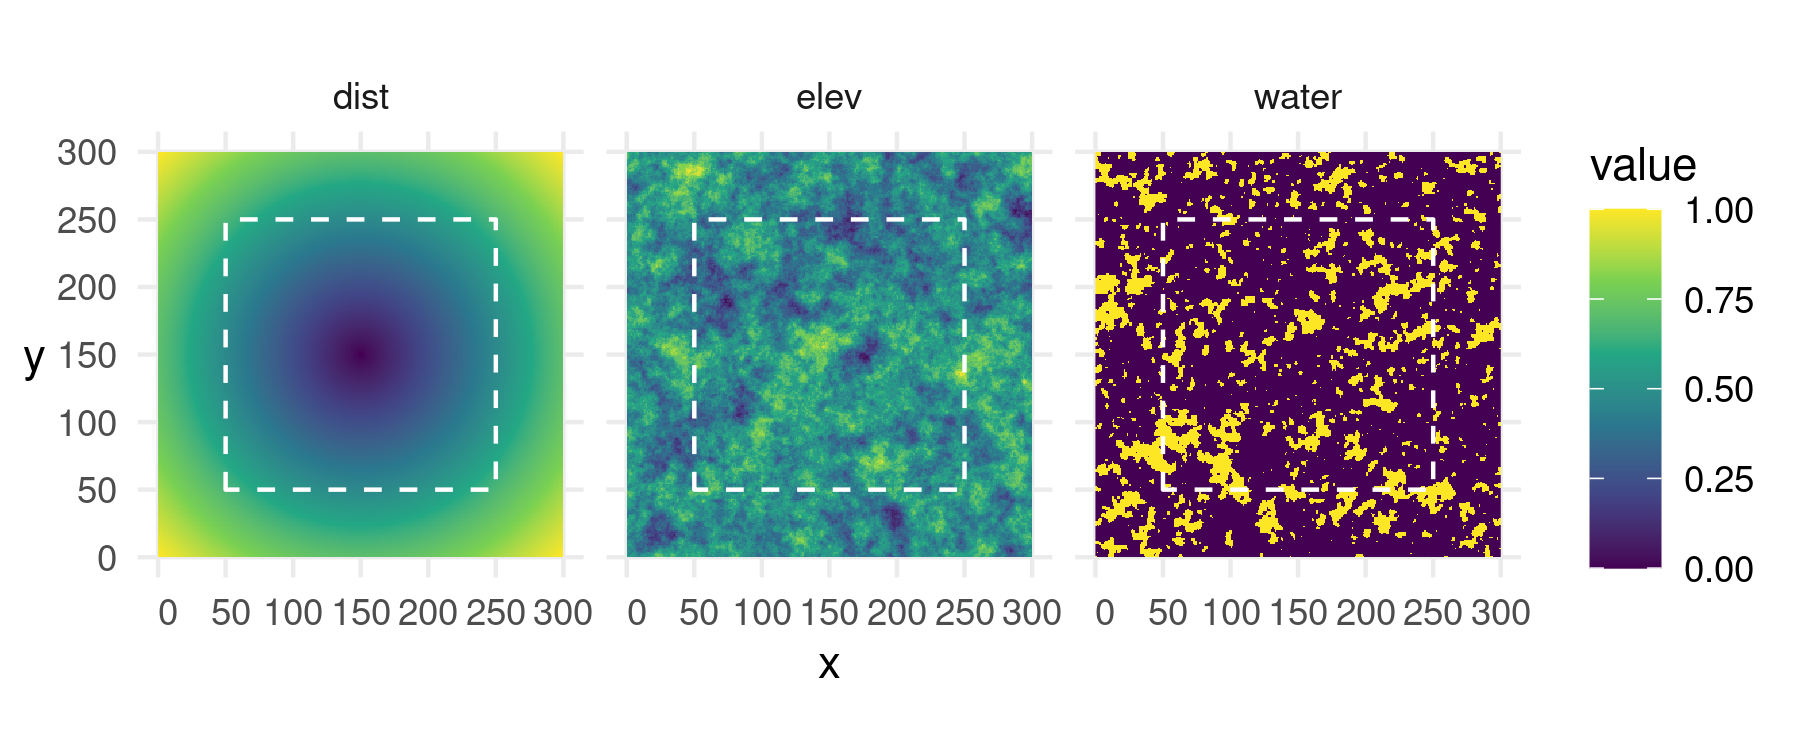
\includegraphics[width = \textwidth]{99_Covariates.png}
  \caption{Virtual landscape across which we simulated movement trajectories.
  All layers have a resolution of 300 x 300 pixels and were generated randomly.
  Simulated individuals were initiated within the white dashed rectangle, which
  ensured that they would not be released directly at a map border.}
  \label{Covariates}
  \end{center}
\end{figure}

\subsubsection{Movement Simulation}
To simulate movement across the above generated virtual lanscape, we employed an
``inverted'' step-selection function, which proceeded as follows. First, we
generated a random starting location. To prevent starting points in the vicinity
of map borders, we restricted sampled locations to x- and y-coordinates between
50 and 250 (white dotted rectangle in \Cref{Covariates}). Second, we generated a
set of 10 random steps originating from the sampled starting point. We then
generated random steps by sampling turning angles from a von Mises distribution
with concentration parameter \(\kappa = 0.5\) and location parameter \( \mu = 0
\), and step lengths from a gamma distribution with shape parameter \(k = 3 \)
and scale parameter \(\theta = 1\). Third, we extracted covariate values along
each random step from the underlying covariate layers and computed the average
of each covariate along every step. Fourth, we predicted for each step the
probability of being chosen by applying \Cref{EQ1}. The vector of relative
habitat preferences used to make predictions was set to \(\beta_{water} = -1\),
\(\beta_{elev} = 0.5\), and \(\beta_{dist} = -15\). Fifth, we sampled one of the
random steps based on predicted probabilities and computed the new position of
the simulated individual. We the repated these steps until a total of 100 steps
were realized and we replicated the simulation 100 times, thus resulting in 100
independent movement trajectories (\Cref{Simulations}). Note that by excluding
interactions among habitat covariates and step metrics we implicitly assume
independent habitat and movement kernels \citep{Avgar.2016}.

\begin{figure}
  \begin{center}
  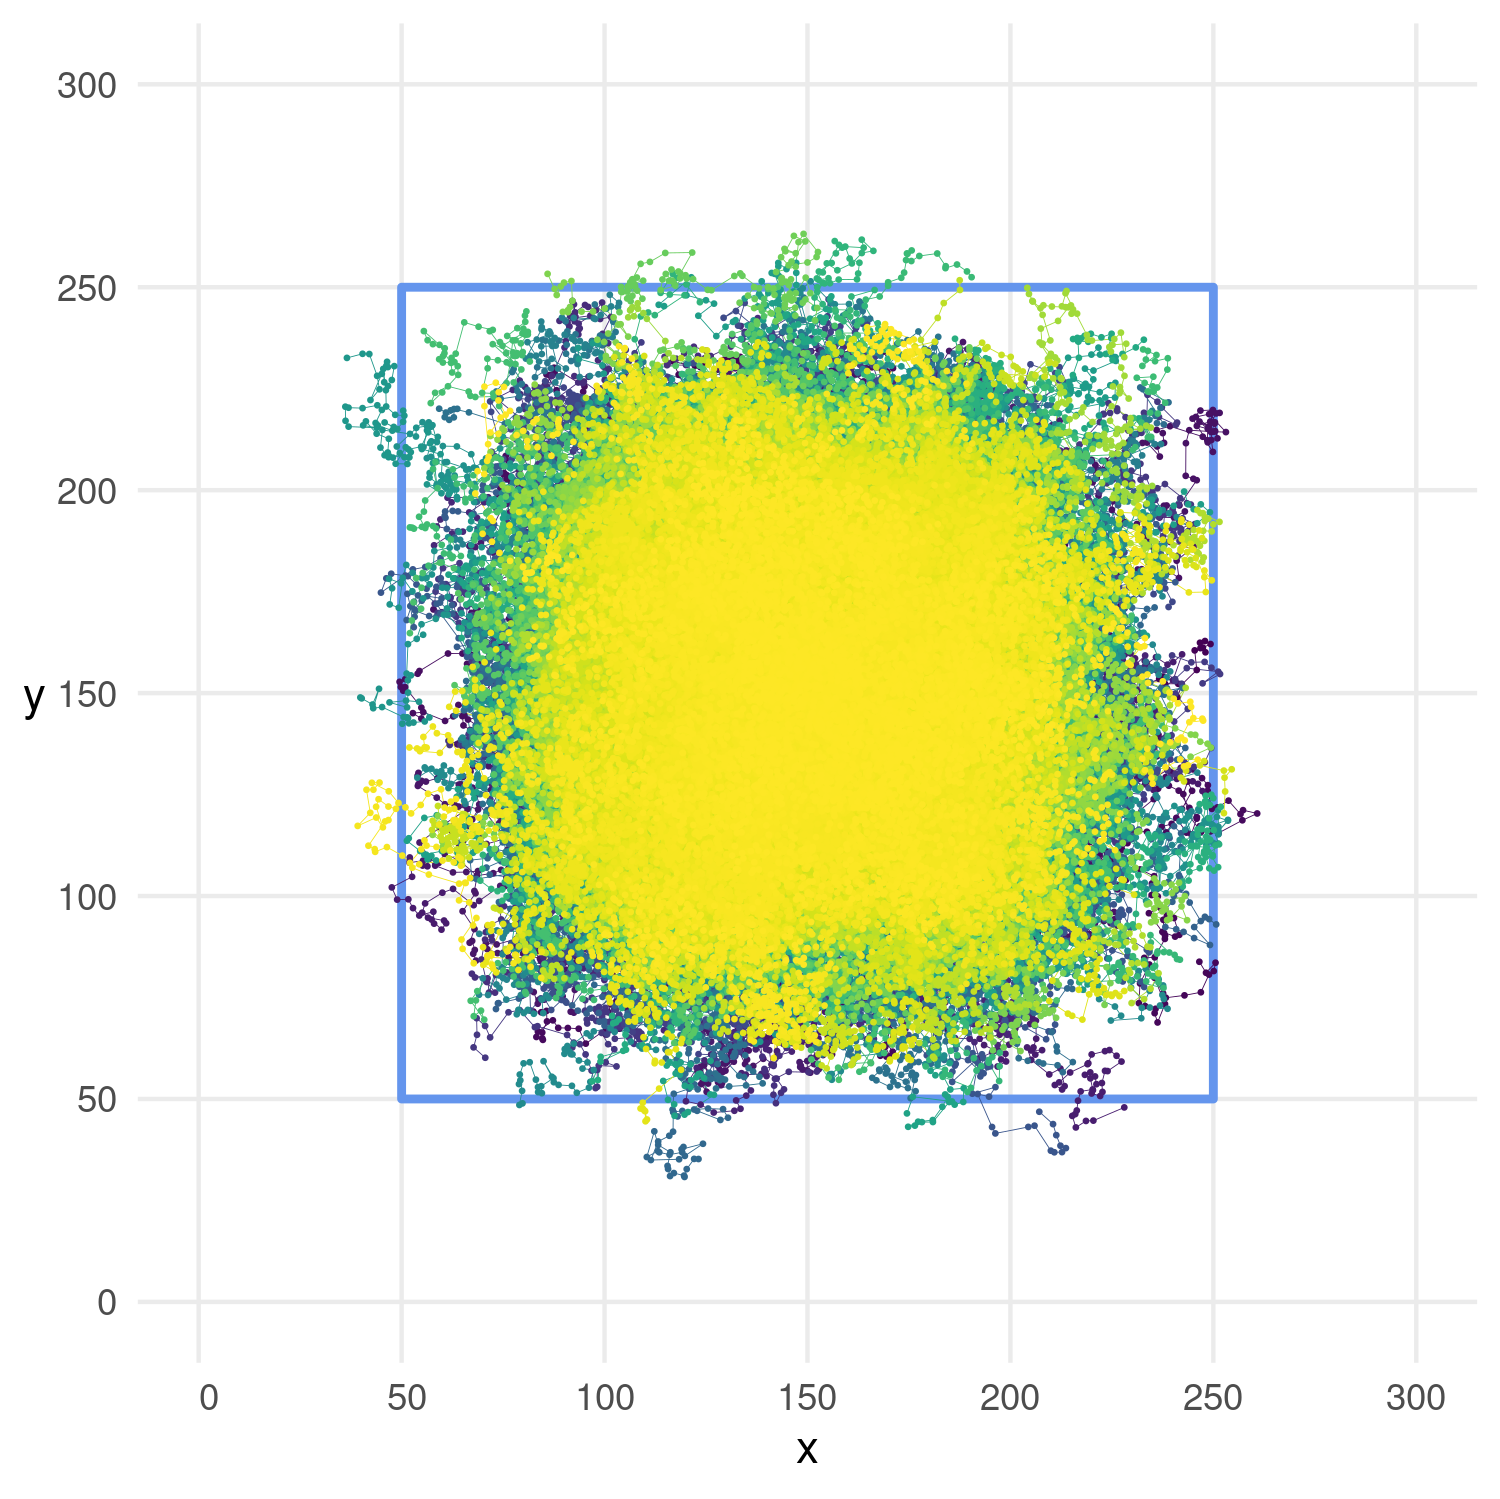
\includegraphics[width = 0.5\textwidth]{99_Simulations.png}
  \caption{100 Simulated movement trajectories, each comprising of 100 steps.
  Simulated individuals were initiated within the blue rectangle to mitigate
  edge effects.}
  \label{Simulations}
  \end{center}
\end{figure}

\subsubsection{Step Selection Analysis}
To assess the consequences of missing GPS data in when employing step-selection
functions, we analysed the simulated GPS data under different conditions
\Cref{Design}. Specifically, we varied the degree of data-missingness (0\% to
80\%), the forgiveness when analysing the data (1 to 5 fixes), and the
parametric distributions from which random steps were generated (static vs.
dynamic distributions). We replicated each combination of conditions 100 times
and computed averages and standard deviations from the resulting model
estimates.

In this context, missingness and forgiveness are complementary terms. While
missingness describes the fraction of data that has not been collected, we use
the term forgiveness to describe how much missingness a modeler is willing to
accept. A modeler with forgiveness of one, for instance, only considers steps
with a step-duration of one (i.e. fixes that are regularly spaced). In contrast,
a modeler with forgiveness of two would also accept steps with a step-duration
of two, thus pardoning a single missing fix.

\paragraph{Data Rarefication}
We rarefied the simulated GPS data by randomly removing a fixed fraction of GPS
fixes. To assess the impact of different degrees of  ``missingness'', we
incrementally increased the fraction of missing fixes from 0.0 (complete
dataset) to 0.8 (80\% missing) with 10\% increments. The removal of GPS fixes
introduced irregular temporal intervals between remaining fixes; we will refer
to these intervals as ``step-times'', where the  ``step'' refers to the straight
line movement between two consecutive GPS fixes \citep{Turchin.1998}. In the
complete dataset, a step-time of one was assumed, whereas the step-time
increased by one for every fix that was missing between subsequent fixes. For
instance, a single missing fix between two other fixes directly increased the
step time from one to two.

\paragraph{Identifying Bursts and Computing Step Metrics}
We used the generated data to compute movement bursts. A movement burst
consisted of a sequence consecutive GPS fixes with step-times that did not
exceed the accepted forgiveness. For instance, if the forgiveness was one,
already a single missing GPS fix introduced a new burst. In contrast, if the
forgiveness was set to two, step-times of two units were allowed, without
introducing a new step.

We will use the term  ``forgiveness'' to indicate how many missing fixes were
accepted before a new burst was enforced. For instance, a forgiveness of one
implied that a single missing fix did not result in a new burst. We then
converted the GPS fixes belonging to the same burst into steps, where each step
resembled the straight line movement between two GPS fixes \citep{Turchin.1998}.
For each step we computed a set of step metrics. This includd the step length,
its logarithm, the turning angle and its cosine.

\paragraph{Step Selection Function}
To conduct step selection analysis, we paired each observed step with 10 random
steps. We generated random steps by sampling turning angles from a von Mises
distribution and step lengths from a gamma distribution. Depending on the study
design, we either sampled turning angles and step lengths from fixed or fixed or
dynamic distributions (cfr. Section ...). Along observed and random steps, we
extracted underlying covariates and computed their averages along steps.

\paragraph{Step Length and Turning Angle Distributions}
To generate random steps, we employed three competing approaches, coined
\textit{uncorrected}, \textit{na\"ive}, and \textit{dynamic} approach,
respectively. In the uncorrected approach, we sampled step-lengths and
turning-angles from parametric gamma and von Mises distributions that were
fitted to observed steps with step-duration of one. In the \textit{na\"ive}
approach, we sampled step lengths and turning angles from the same
distributions, yet we linearly scaled sampled step lengths to the actual
step-duration. For instance, for any step with a step-duration of two, we
doubled the sampled step length. This approach is representative of the
time-varying SSF approach proposed by \cite{Munden.2021}. Finally, in the
\textit{dynamic} approach, we sampled step lengths and turning angles from
distributions that were fit to different step-durations. That is, we fitted
separate step length and turning angles distributions to every possible step
duration. To achieve this, we subsampled the observed data to 50\% of the fixes,
which resulted in varying step-durations. We then and fitted step length and
turning angle distributions to the steps from different step-durations. We
repeated this procedure 1000 times and averaged the parameter estimates across
replicates.

\paragraph{Regression Model}
We estimated ... using conditional logistic regression, implemented using the
r-package \textsf{survival} \citep{Therneau.2021}. We followed \cite{Avgar.2016}
and \cite{Fieberg.2021} and employed \textit{integrated} SSA. That is, aside
from the habitat covariates (\textsf{water, elev, dist}), we also included
descriptors of the step length and turning angle (\textsf{sl, log(sl), cos(ta)})
in our regression model. The model call was as follows:

$$
case\_ \sim water + elev + dist + sl + log(sl) + cos(ta)
$$

\subsection{Case Study}

because wild dogs move comparably little in the hours between xx and xx, we made
the simplyfing assumption that the 8-hour period from xx to xx is comparable to
a 4-hour period.


\section{Results}
\section{Discussion}
Results from our simulation study demonstrate that the inclusion of GPS fixes
can be used to gain information on relative habitat preferences of the focal
species. While the inclusion of steps from irregular sampling schemes resulted
in substantial biases for estimates related to step metrics, we showed that
these biases can effectively be mitigated by generating step lengths and turning
angles from distributions that are separately fit to steps from different step
durations. Regardless of biases in beta coefficients for step metrics, we found
that habitat selection estimates were unbiased, even when including irregular
steps. Even more, the inclusion of irregular steps drastially reduced model
uncertainty, thus suggesting that such data can be used to gain information that
would otherwise be lost.

\section{Authors' Contributions}
D.D.H., D.M.B., A.O. and G.C. conceived the study and designed methodology;
D.M.B., G.C., and J.W.M. collected the data; D.D.H. and D.M.B. analysed the
data; G.C. and A.O. assisted with modeling; D.D.H., D.M.B., and G.C. wrote the
first draft of the manuscript and all authors contributed to the drafts at
several stages and gave final approval for publication.

\section{Data Availability}
GPS movement data of dispersing wild dogs is available on dryad
\citep{Hofmann.2021b}. Access to R-scripts that exemplify the application of the
proposed approach using simulated data are provided through Github
(\url{https://github.com/DavidDHofmann/DispersalSimulation}). In addition, all
codes required to reproduce the African wild dog case study will be made
available through an online repository at the time of publication.

\section{Acknowledgements}
We thank the Ministry of Environment and Tourism of Botswana for granting
permission to conduct this research. We thank C. Botes, I. Clavadetscher, and G.
Camenisch for assisting with wild dog immobilizations. We also thank B. Abrahms
for sharing her data of three dispersing wild dogs. Furthermore, we would like
to thank Johannes Signer for assisting with the simulation algorithm. This study
was funded by Albert-Heim Foundation, Basler Stiftung für Biologische Forschung,
Claraz Foundation, Idea Wild, Jacot Foundation, National Geographic Society,
Parrotia Stiftung, Stiftung Temperatio, Wilderness Wildlife Trust Foundation,
Forschungkredit der Universität Zürich, and a Swiss National Science Foundation
Grant (31003A\_182286) to A. Ozgul.

\newpage
\begingroup
\singlespacing
\bibliography{Literatur}
\endgroup

\end{document}
